\subsection{de.view.elements.theme}

\rule{\textwidth}{0.4pt} 
\class{ColorTheme}
public abstract class ColorTheme

\begin{minipage}{0.3\textwidth}
    \begin{figure}[H]
        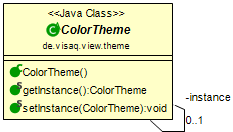
\includegraphics[scale = 0.5]{media/frontend/view/de.view.elements.theme/ColorTheme_Class.png}
    \end{figure}
    \end{minipage} \hfill
    \begin{minipage}{0.6\textwidth}
ColorTheme ist eine Funktion mit welcher der Benutzer die Farben wechseln kann in welchen die Schnittstelle dargestellt wird. Die Klasse wurde nach einem Singelton Entwurfsmuster designt
\end{minipage}

Methoden:
\begin{itemize} 
    \item \emph{public ColorTheme()} Erstellt eine ColorTheme Instanz und aktualisiert diese.
    \item \emph{public static synchronized ColorTheme getInstance()} Gibt einen Wert von dem Typ ColorTheme zurück
    \item \emph{public static synchronized void setInstance(ColorTheme colorTheme)} Setzt die aktuelle ColorTheme Instanz   
    \item \emph{public abstract Gradient getPrimarySkala()} Gibt einen Wert von dem Typ Gradient zurück
    \item \emph{public abstract Gradient getSecondarySkala()}  Gibt einen Wert von dem Typ Gradient zurück
\end{itemize}

\rule{\textwidth}{0.4pt} 
\class{DarkTheme}
public class DarkTheme extends ColorTheme

\begin{minipage}{0.3\textwidth}
    \begin{figure}[H]
        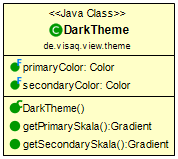
\includegraphics[scale = 0.5]{media/frontend/view/de.view.elements.theme/DarkTheme_Class.png}
    \end{figure}
    \end{minipage} \hfill
    \begin{minipage}{0.6\textwidth}
       Ein dunkleres Farbschema für die Visualisierung der Website.
    \end{minipage}

Methoden:
\begin{itemize} 
    \item \emph{public ColorTheme()} Erstellt eine ColorTheme Instanz und aktualisiert diese.
    \item \emph{public static synchronized ColorTheme getInstance()} Gibt einen Wert von dem Typ ColorTheme zurück
    \item \emph{public static synchronized void setInstance(ColorTheme colorTheme)} Setzt die aktuelle ColorTheme Instanz    \item \emph{public abstract Gradient getPrimarySkala()} Gibt einen Wert von dem Typ Gradient zurück
    \item \emph{public abstract Gradient getSecondarySkala()}  Gibt einen Wert von dem Typ Gradient zurück
\end{itemize}

\rule{\textwidth}{0.4pt} 
\class{LightTheme}
public class LightTheme extends ColorTheme

\begin{minipage}{0.3\textwidth}
    \begin{figure}[H]
        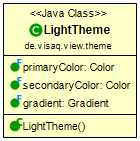
\includegraphics[scale = 0.5]{media/frontend/view/de.view.elements.theme/LightTheme_Class.png}
    \end{figure}
    \end{minipage} \hfill
    \begin{minipage}{0.6\textwidth}
        Ein helleres Farbschema für die Visualisierung der Website. Diese wird bei einem Erstbesuch als Standardschema geladen.
    \end{minipage}

Methoden:
\begin{itemize} 
    \item \emph{public ColorTheme()} Erstellt eine ColorTheme Instanz und aktualisiert diese.
    \item \emph{public static synchronized ColorTheme getInstance()} Gibt einen Wert von dem Typ ColorTheme zurück
    \item \emph{public static synchronized void setInstance(ColorTheme colorTheme)} Setzt die aktuelle ColorTheme Instanz    \item \emph{public abstract Gradient getPrimarySkala()} Gibt einen Wert von dem Typ Gradient zurück
    \item \emph{public abstract Gradient getSecondarySkala()}  Gibt einen Wert von dem Typ Gradient zurück
\end{itemize}

\rule{\textwidth}{0.4pt} 
\class{ColorBlindTheme}
public class ColorBlindTheme extends ColorTheme

\begin{minipage}{0.3\textwidth}
\begin{figure}[H]
    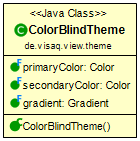
\includegraphics[scale = 0.5]{media/frontend/view/de.view.elements.theme/ColorBlindTheme_Class.png}
\end{figure}
\end{minipage} \hfill
\begin{minipage}{0.6\textwidth}
    Ein Farbblindenschema für die Visualisierung der Website. In diesem Fall speziell für eine Rot-Grün Sehschwäche.
\end{minipage}

Methoden:
\begin{itemize} 
    \item \emph{public ColorTheme()} Erstellt eine ColorTheme Instanz und aktualisiert diese.
    \item \emph{public static synchronized ColorTheme getInstance()} Gibt einen Wert von dem Typ ColorTheme zurück
    \item \emph{public static synchronized void setInstance(ColorTheme colorTheme)} Setzt die aktuelle ColorTheme Instanz
    \item \emph{public abstract Gradient getPrimarySkala()} Gibt einen Wert von dem Typ Gradient zurück
    \item \emph{public abstract Gradient getSecondarySkala()}  Gibt einen Wert von dem Typ Gradient zurück
\end{itemize}

\rule{\textwidth}{0.4pt} 
\class{Gradient} 
public class Gradient

\begin{minipage}{0.3\textwidth}
    \begin{figure}[H]
    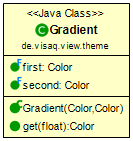
\includegraphics[scale = 0.5]{media/frontend/view/de.view.elements.theme/Gradient_Class.png}
    \end{figure}
    \end{minipage} \hfill
    \begin{minipage}{0.6\textwidth}
    Beschreibt einen Farbverlauf zwischen zwei Punkten. Und kann auf die spezifischen Farbwerte im Farbverlauf zugreifen.
    \end{minipage}

    Attribute:
\begin{itemize} 
    \item \emph{public final Color first} Die Primärfarbe für das erstellen des Farbverlaufs.
    \item \emph{public final Color second} Die Sekundärfarbe für das erstellen des Farbverlaufs.
\end{itemize}
Methoden:
\begin{itemize} 
    \item \emph{public Gradient(Color first, Color second)} Konstruktor, welcher mithilfe der Primärfarbe und Sekundärfarbe den Farbverlauf erstellt.
    \item \emph{public Color get(float at)} Gibt eine Farbe zurück, welche zwischen * 100 Prozent der Primärfarbe und Sekundärfarbe liegt und mithilfe von linearer Interpolation.
\end{itemize}